\documentclass[a4paper,12pt]{article}

\usepackage[T1]{fontenc}
\usepackage[utf8]{inputenc}
\usepackage[english, polish]{babel}
\usepackage{lmodern}
\usepackage{graphicx}
\usepackage{fancyhdr}
\usepackage{float}
\usepackage{array}
\usepackage{hyperref}
%\usepackage{mathtools}


\setlength{\textheight}{23.5cm}
\setlength{\textwidth}{15.92cm}
\setlength{\footskip}{10mm}
\setlength{\oddsidemargin}{0mm}
\setlength{\evensidemargin}{0mm}
\setlength{\topmargin}{0mm}
\setlength{\headsep}{15mm}
\setlength{\parindent}{0cm}
\setlength{\parskip}{2.5mm}
%nowa extra row do tabeli :)  :) 
\setlength{\extrarowheight}{4pt}

\author{Justyna Ilczuk, Jacek Rosiński}

\begin{document}

\begin{center}

    \begin{tabular}{ | m{5cm}| m{5cm} | m{5cm} |}
    \hline 
    \multicolumn{2}{|c|}{{ \Large \textbf{Laboratorium Fizyki 2}} }
    &  
    \begin{center}
    Data wykonania ćwiczenia:
    \end{center}
    \begin{center}
      16.10.2013 
    \end{center}
    \begin{center}
    Środa 9.45-13.45
    \end{center}
     \\ 
    
    \hline
    \multicolumn{2}{|c|}{Justyna Ilczuk \newline Jacek Rosiński}
    & \begin{center}
    {\small Data złożenia sprawozdania:} \newline \today
    \end{center}   \\
   	
   	\hline
    Wydział Fizyki & Grupa: K-1 \newline Rok akademicki: 2013/2014 &  \\
   	\hline
   	\multicolumn{2}{|l|}{Prowadzący: Michał Marzanotowicz} & \multicolumn{1}{|l|}{Ocena końcowa:}\\
    \hline
    \end{tabular}
\end{center}

\newpage

\pagestyle{fancy}
\fancyfoot[CO]{\ }
\fancyhead[RO]{\footnotesize{\thepage} }
%\fancyhead[RO]{\footnotesize{\ } }
\fancyhead[LO]{Justyna Ilczuk i Jacek Rosiński K-1, Diody fotowoltaiczne }

% wrzucanie wykresów:

%\begin{figure} [H]
%  \begin{center}
%    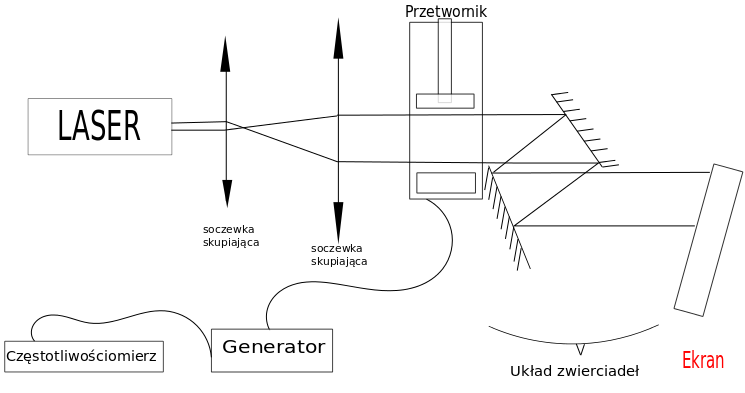
\includegraphics[width = 15cm]{Rysunek.png}
%    \caption{Układ pomiarowy}
%  \end{center}
%\end{figure}


\section{Cel ćwiczenia}
Pomierzyć sobie próbki i zobaczyć i zrozumieć co tam się fajnego w środku dzieje.

\section{Przebieg laboratoriów}
Czyli co badaliśmy na których i co nam się udało i jakie mieliśmy problemy.


\section{Wyniki pomiarów}

Dla jednej próbki mierzyliśmy charakterystyki jasne i ciemne.
Dla drugiej próbki mierzyliśmy tylko charakterystyki jasne.

A dla trzeciej próbki liczylismy koncentrację nośników (dziur chyba?).

Poniżej przedstawiamy wykresy charakterystyk diod w zależnosci od temperatury dla dwóch badanych próbek.

\begin{figure} [H]
  \begin{center}
    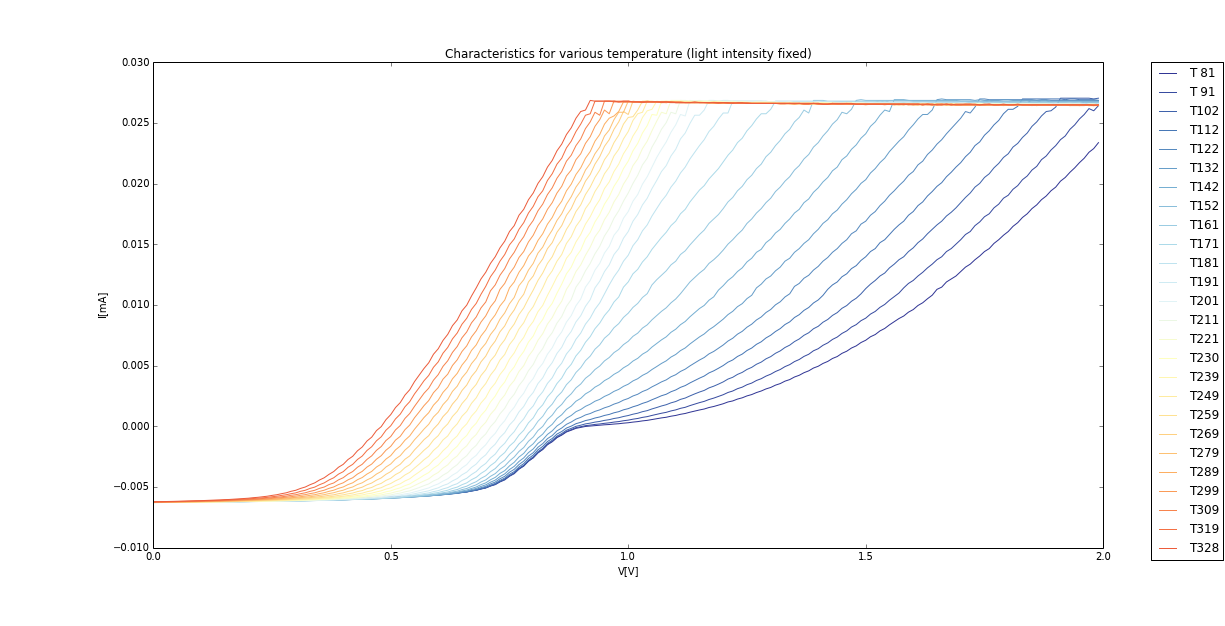
\includegraphics[width = 15cm]{probka1_temperatura.png}
    \caption{Próbka 1 - charakterystyki dla różnych temperatur}
  \end{center}
\end{figure}

\begin{figure} [H]
  \begin{center}
    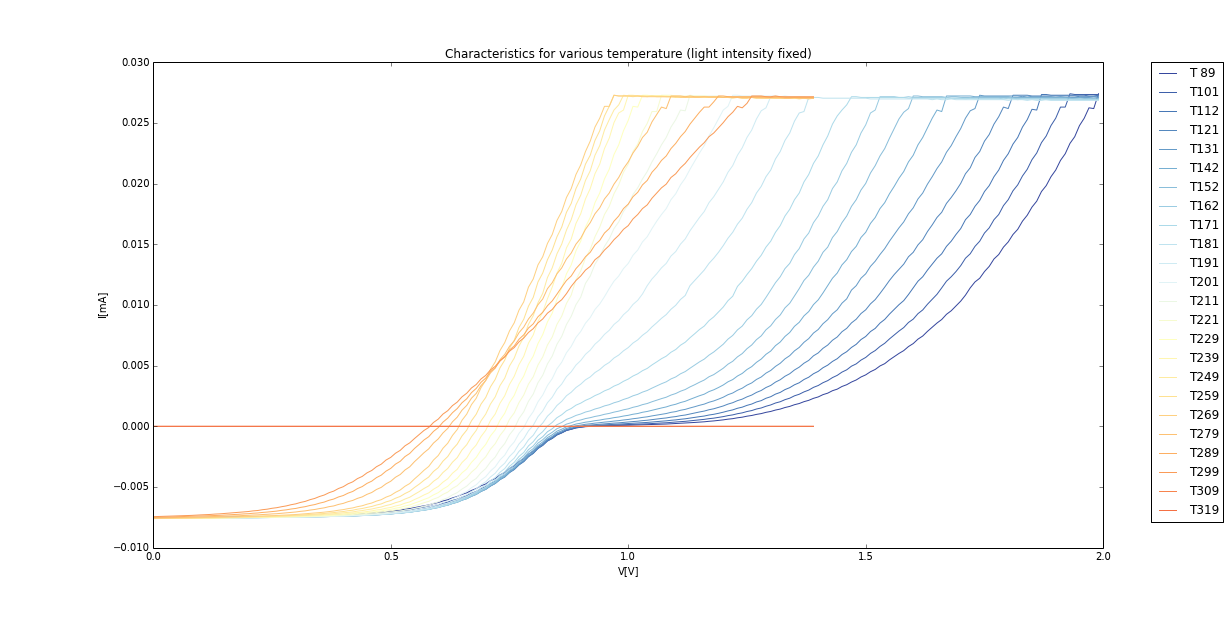
\includegraphics[width = 15cm]{probka2_temperatura.png}
    \caption{Próbka 2 - charakterystyki dla różnych temperatur}
  \end{center}
\end{figure}


Dalej przedstawiamy wykresy dla różnych wartości natężeń światła.
\begin{figure} [H]
  \begin{center}
    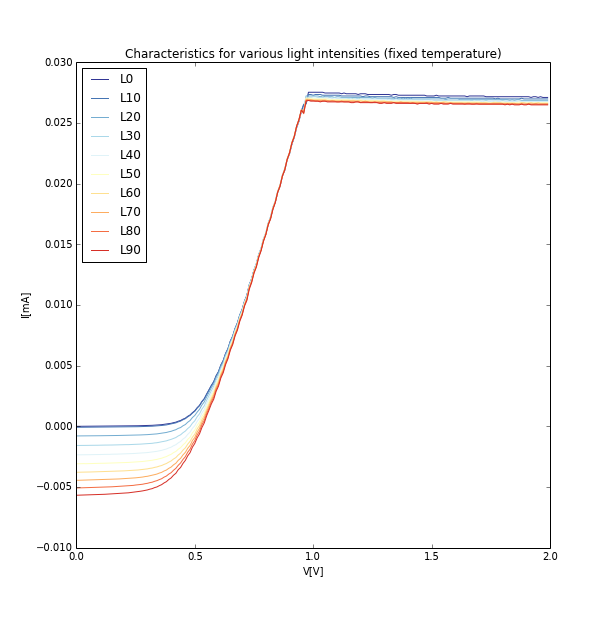
\includegraphics[width = 15cm]{probka1_swiatlo.png}
    \caption{Próbka 1 - charakterystyki dla różnych natężeń światła}
  \end{center}
\end{figure}

\begin{figure} [H]
  \begin{center}
    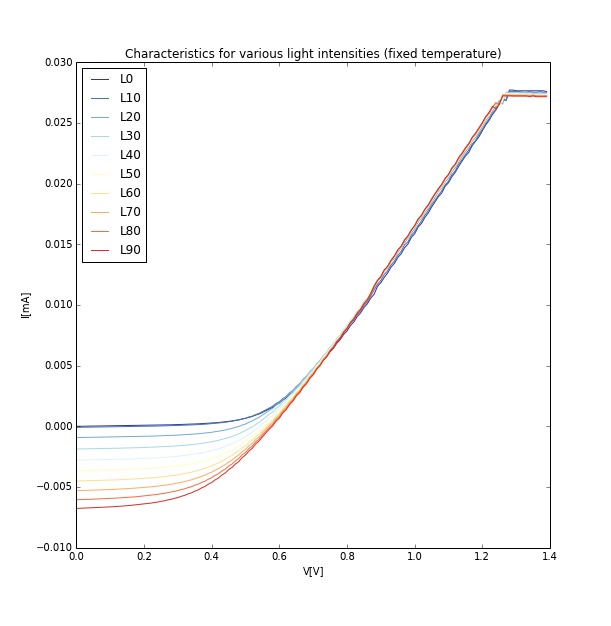
\includegraphics[width = 15cm]{probka2_swiatlo.png}
    \caption{Próbka 1 - charakterystyki dla różnych natężeń światła}
  \end{center}
\end{figure}

Dalej przedstawiamy na zbioryczych wykresach kilka parametrów naszych próbek:

\begin{figure} [H]
  \begin{center}
    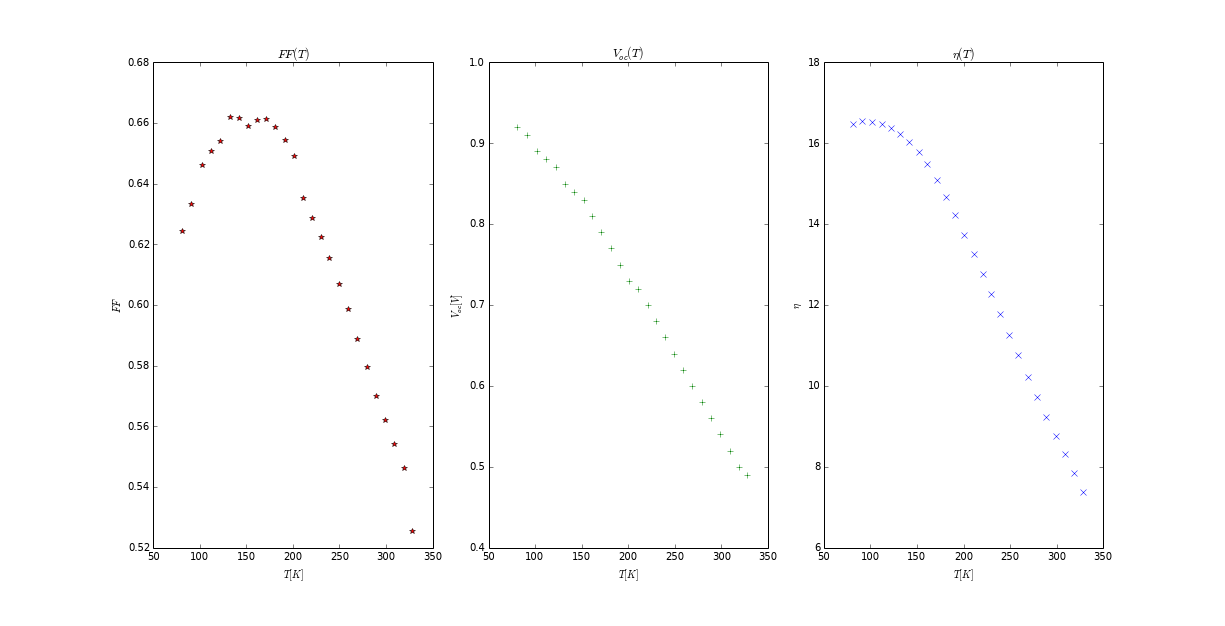
\includegraphics[width = 15cm]{probka1_rozne.png}
    \caption{Parametry próbki 1}
  \end{center}
\end{figure}

\begin{tabular}{lrrrrrr}

{} &          pmax &        ff &        eta &  V\_oc &  temp &  intensity \\

1   &  3.876000e-03 &  0.559204 &  17.889368 &  0.92 &   101 &        100 \\
12  &  3.940720e-03 &  0.573799 &  18.188078 &  0.91 &   112 &        100 \\
23  &  3.985980e-03 &  0.586372 &  18.396972 &  0.90 &   121 &        100 \\
34  &  4.012640e-03 &  0.596452 &  18.520019 &  0.89 &   131 &        100 \\
45  &  4.020080e-03 &  0.603869 &  18.554358 &  0.88 &   142 &        100 \\
56  &  4.027520e-03 &  0.611456 &  18.588697 &  0.87 &   152 &        100 \\
67  &  4.023800e-03 &  0.625265 &  18.571527 &  0.85 &   162 &        100 \\
78  &  4.008920e-03 &  0.636954 &  18.502850 &  0.83 &   171 &        100 \\
89  &  3.982200e-03 &  0.640425 &  18.379526 &  0.82 &   181 &        100 \\
100 &  3.938400e-03 &  0.648190 &  18.177371 &  0.80 &   191 &        100 \\
111 &  3.861000e-03 &  0.643495 &  17.820137 &  0.79 &   201 &        100 \\
122 &  3.760720e-03 &  0.643061 &  17.357303 &  0.77 &   211 &        100 \\
133 &  3.603600e-03 &  0.632627 &  16.632128 &  0.75 &   221 &        100 \\
144 &  3.498120e-03 &  0.630934 &  16.145293 &  0.73 &   229 &        100 \\
155 &  3.368560e-03 &  0.624188 &  15.547320 &  0.71 &   239 &        100 \\
166 &  3.217500e-03 &  0.613962 &  14.850114 &  0.69 &   249 &        100 \\
177 &  3.068640e-03 &  0.603036 &  14.163063 &  0.67 &   259 &        100 \\
188 &  2.906740e-03 &  0.589728 &  13.415826 &  0.65 &   269 &        100 \\
199 &  2.564520e-03 &  0.539375 &  11.836337 &  0.63 &   279 &        100 \\
210 &  2.281200e-03 &  0.498756 &  10.528696 &  0.61 &   289 &        100 \\
221 &  2.037600e-03 &  0.464001 &   9.404380 &  0.59 &   299 &        100 \\
232 &  2.041179e-08 &  0.201465 &   0.000094 &  0.50 &   309 &        100 \\
243 &  9.407765e-09 &  0.201282 &   0.000043 &  0.39 &   319 &        100 \\
254 &  3.766200e-03 &  0.537949 &  17.382595 &  0.93 &    89 &        100 \\

\end{tabular}

\begin{figure} [H]
  \begin{center}
    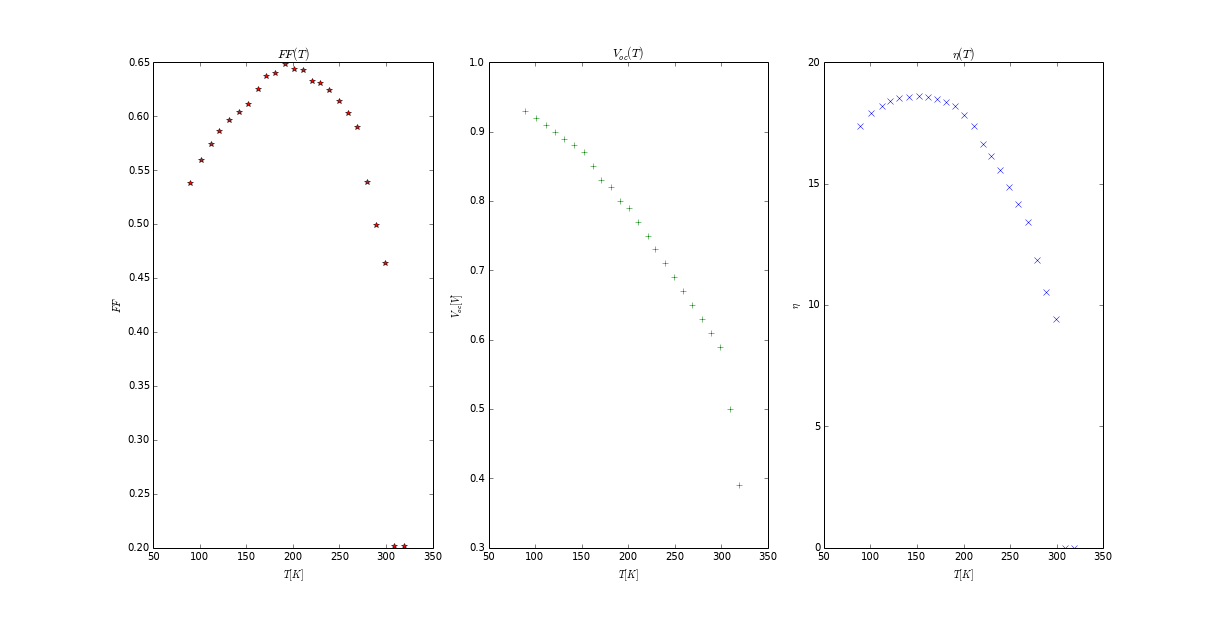
\includegraphics[width = 15cm]{probka2_rozne.png}
    \caption{Parametry próbki 2}
  \end{center}
\end{figure}

Dalej porównujemy poszczególne parametry pomiędzy próbkami:

\begin{figure} [H]
  \begin{center}
    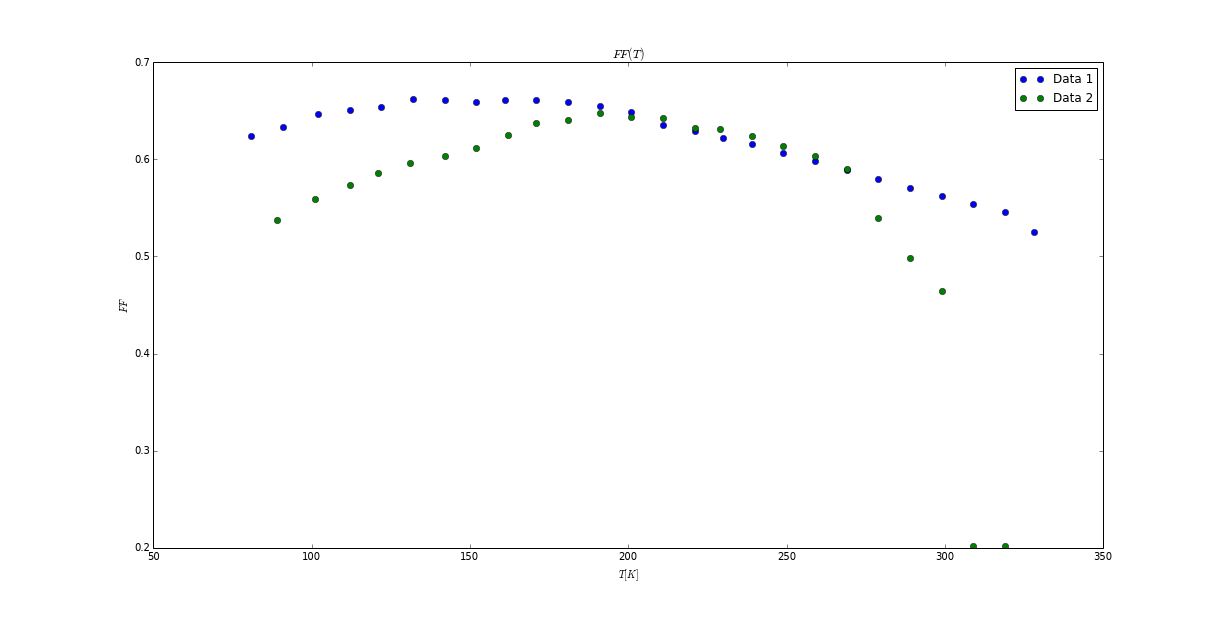
\includegraphics[width = 15cm]{probki_porownanie_FF.png}
    \caption{Porównanie FF}
  \end{center}
\end{figure}

\begin{figure} [H]
  \begin{center}
    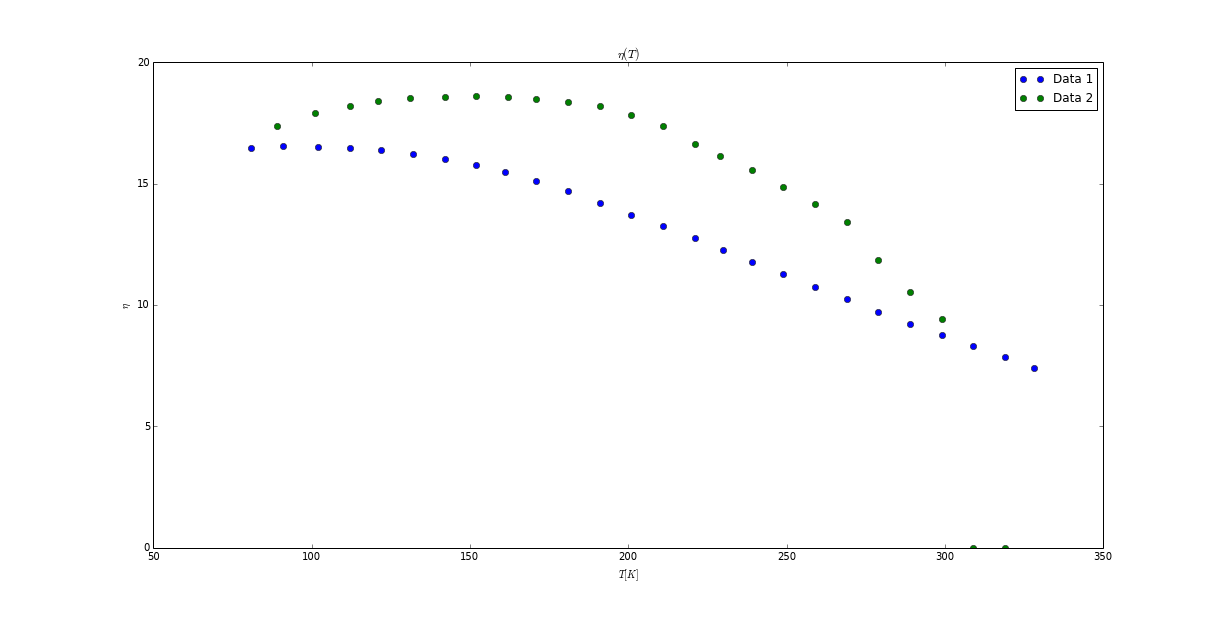
\includegraphics[width = 15cm]{probki_porownanie_eta.png}
    \caption{Porównanie $\eta$}
  \end{center}
\end{figure}

\begin{figure} [H]
  \begin{center}
    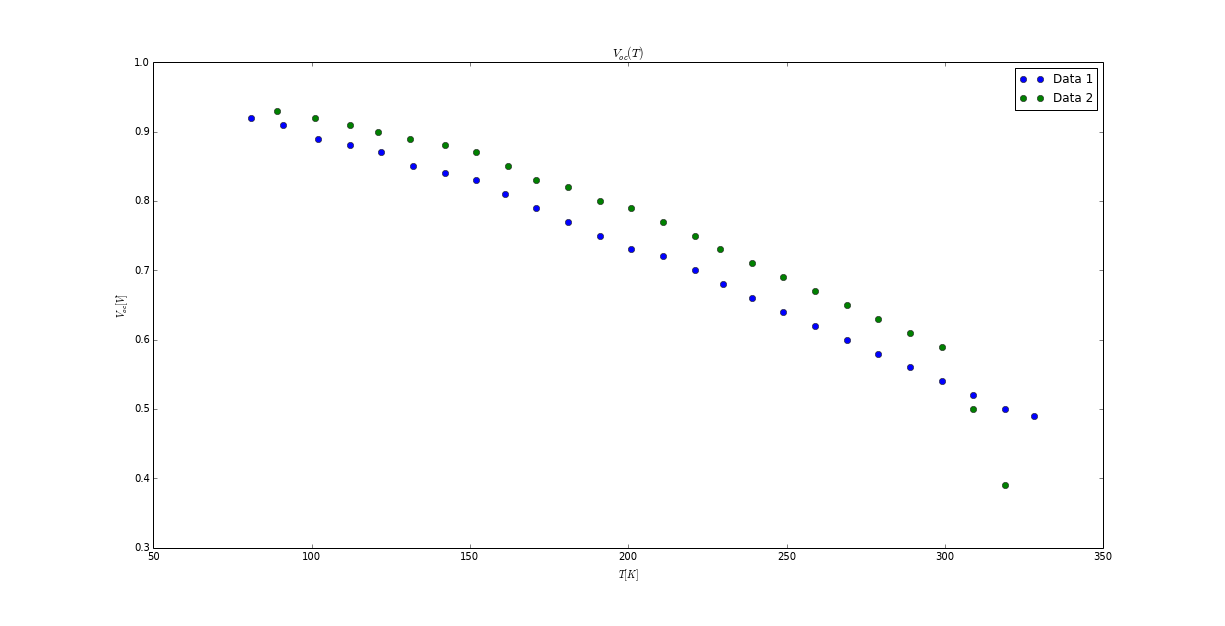
\includegraphics[width = 15cm]{probki_porownanie_V_oc.png}
    \caption{Porównanie $V_{oc}$}
  \end{center}
\end{figure}





Dopasowując prostą do $V_{oc}$ można wyliczyć  $\Phi_b$
\begin{figure} [H]
  \begin{center}
    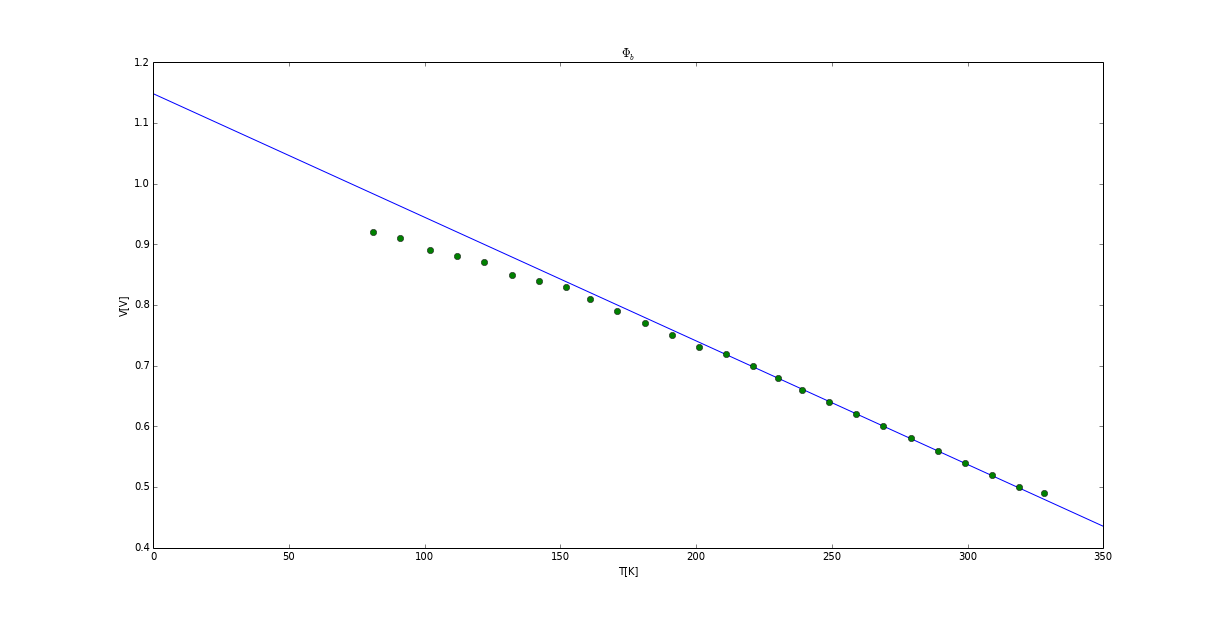
\includegraphics[width = 15cm]{probka1_phi_b.png}
    \caption{$\Phi_b$ dla pierwszej próbki}
  \end{center}
\end{figure}

\begin{figure} [H]
  \begin{center}
    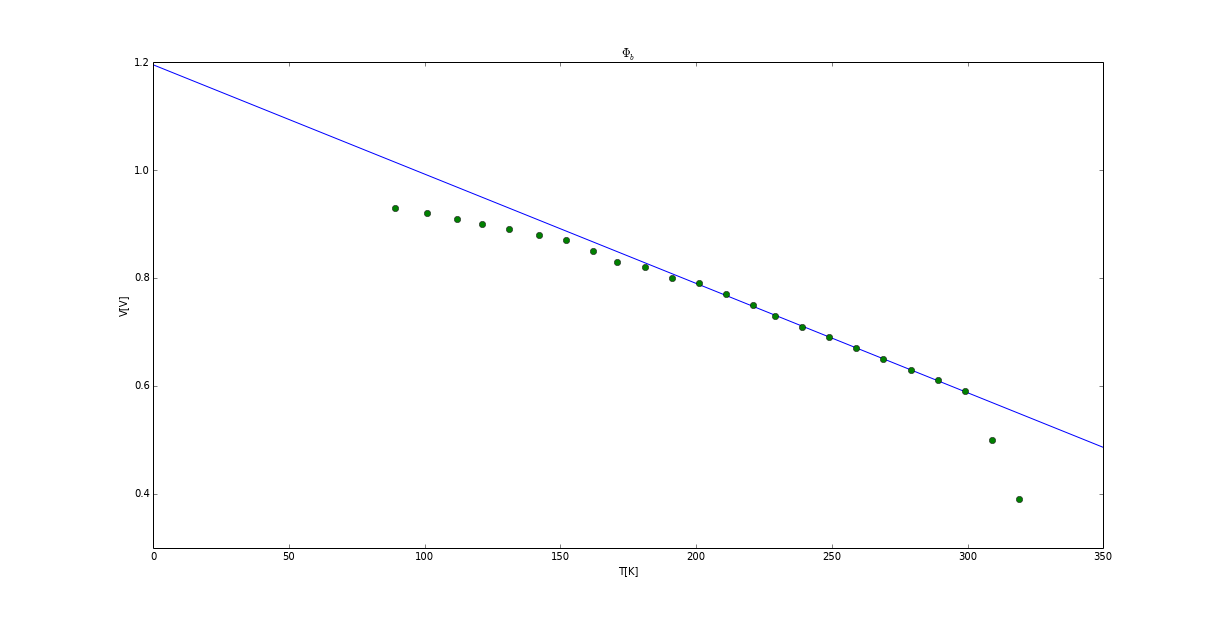
\includegraphics[width = 15cm]{probka2_phi_b.png}
    \caption{$\Phi_b$ dla drugiej próbki}
  \end{center}
\end{figure}

Dla pierwszej próbki:

$$\Phi_b = 1.15$$

Dla drugiej próbki:

$$\Phi_b = 1.20$$

I to tyle jeśli chodzi o wykresy dla jasnych charakterystyk.

Dla pierwszej próbki zbadaliśmy ciemne charakterystyki.

Oto co zaobserwowaliśmy:
\begin{figure} [H]
  \begin{center}
    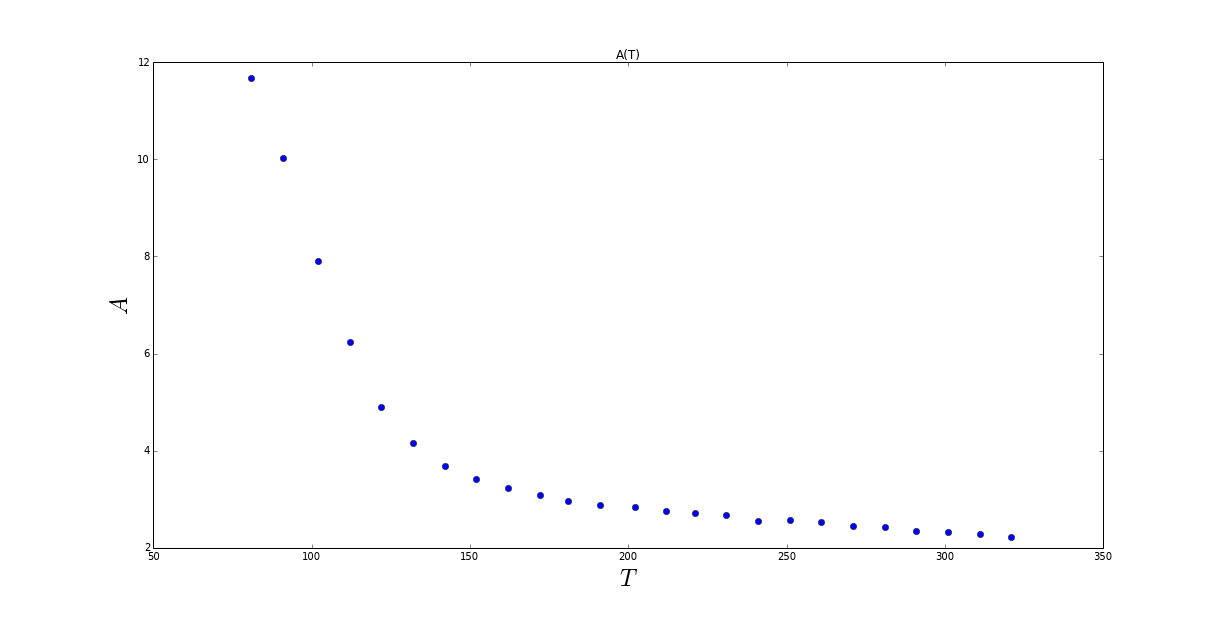
\includegraphics[width = 15cm]{A_T.png}
    \caption{A(T)}
  \end{center}
\end{figure}

Przekształcając zależność:

tu wzorek z Joo i A. Otrzymujemy:

W ten sposób wyznaczamy $\Phi_b$ dla pierwszej próbki.


$$\Phi_b = 1.16$$

\begin{figure} [H]
  \begin{center}
    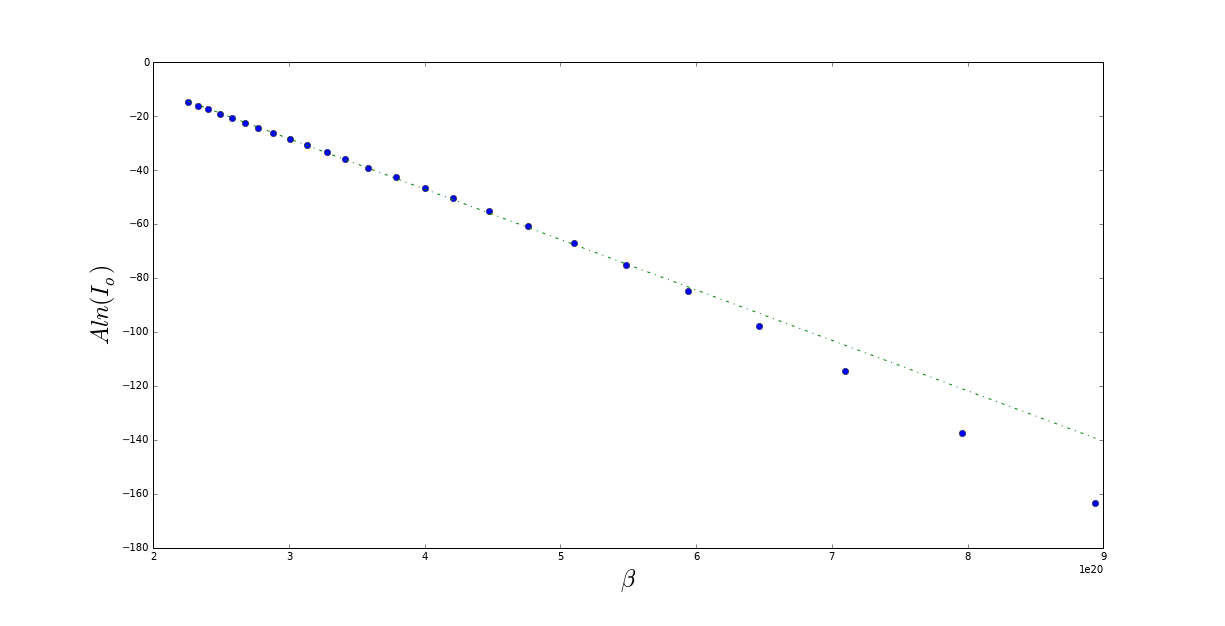
\includegraphics[width = 15cm]{A_lnI.png}
    \caption{A ln(I)}
  \end{center}
\end{figure}
\section{Wstęp}

\section{Wnioski}


\end{document}
